\chapter{化学反应：反应物与生成物}\label{ch:g7:chemical-reactions}

木炭在烧烤炉中发出红光。一小时后，黑色的炭块几乎全部
消失了，只剩下少量灰色的灰烬，以及烤熟食物的热量。
黑色的碳去哪儿了？它并没有消失，而是
与空气中的氧气结合，变成了一种看不见的新气体。
掌握了原子和分子的知识，我们现在就能准确说明这类变化中究竟发生了什么。

\begin{recall}
在化学变化中，会生成新物质，且
无法简单复原（见\cref{ch:g5:irreversible-changes}）。石灰水遇二氧化碳变浑浊，
无水硫酸铜遇水变蓝
（见\cref{ch:g7:identifying-substances}）。一切物质都由原子构成，
原子结合成分子；化学式如 \ce{CO2} 列出的是一个分子中
所含原子的种类和数目（见\cref{ch:g7:atoms-and-molecules}）。
\end{recall}

\begin{omfigure}
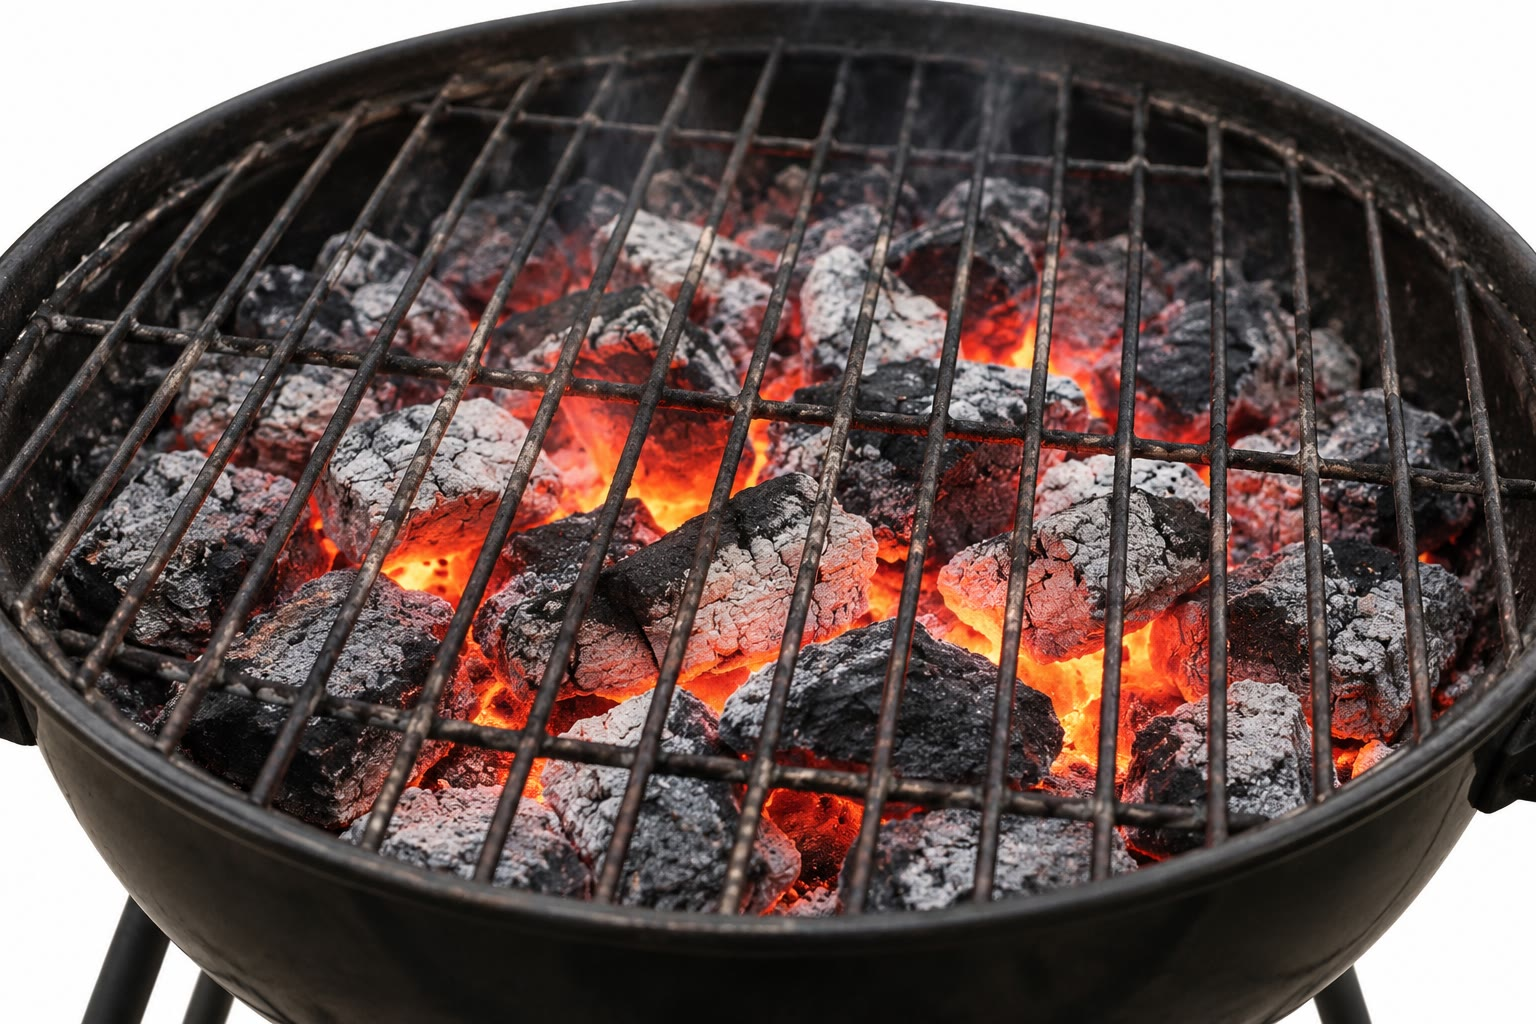
\includegraphics[width=0.55\linewidth]{images/book1/ai/g7-charcoal-bbq.jpg}

{\small 发光的木炭：碳与空气中的氧气发生反应。}
\end{omfigure}

\section{物理变化与化学变化}

\begin{definition}[物理变化]\label{def:g7:chemical-reactions:physical-transformation}
\emph{物理变化}\index{物理变化}是指在不改变化学物种的前提下，
改变物质的状态或排列方式，例如熔化、凝固、
沸腾、溶解、混合。变化前后的
化学物种相同，
只是它们的形态或排列方式发生了改变。
\end{definition}

\begin{example}[水的三种变化]\label{ex:g7:chemical-reactions:water}
冰熔化成水、水沸腾变成水蒸气，以及食盐
溶于水，均属物理变化：变化前后
都存在水分子（以及食盐）。放大来看，分子
本身没有改变，只是它们的排列方式和运动情况发生了变化。
\end{example}

\begin{proposition}[化学变化]\label{prop:g7:chemical-reactions:chemical}
在化学变化中，某些
化学物种消失，同时生成新的化学物种。化学变化与物理变化的区别在于
其生成物中出现了新的化学物种，
可以通过特征检验加以检出。
\end{proposition}

\begin{omfigure}
\begin{tikzpicture}[font=\small, level distance=1.5cm,
    box/.style={draw=omDef, fill=omDef!6, rounded corners=2pt, align=center,
      inner sep=4pt},
    level 1/.style={sibling distance=6.6cm},
    edge from parent/.style={draw, thick, omDef, ->}]
  \node[box] {物质的变化}
    child {node[box, text width=5.2cm] {\textbf{物理}：化学物种 \\
      前后相同 \\ \footnotesize 熔化、沸腾、溶解、混合}}
    child {node[box, draw=omProp, fill=omProp!6, text width=5.2cm]
      {\textbf{化学}：化学物种消失，\\ 生成新物种 \\
      \footnotesize 燃烧、生锈、烹饪}};
\end{tikzpicture}

{\small 两类变化。}
\end{omfigure}

\section{反应物与生成物}

\begin{definition}[化学反应]\label{def:g7:chemical-reactions:reaction}
\emph{化学反应}\index{化学反应}是化学家用来描述化学变化的模型，
它列出了被消耗的化学物种
以及生成的化学物种。
\end{definition}

\begin{definition}[反应物与生成物]\label{def:g7:chemical-reactions:reactant}
在化学反应中被消耗的化学物种称为
\emph{反应物}\index{反应物}；生成的化学物种称为
\emph{生成物}\index{生成物}。
\end{definition}

\begin{example}[碳在氧气中燃烧]\label{ex:g7:chemical-reactions:carbon}
木炭燃烧时，反应物是碳（即木炭）和氧气
（来自空气）。生成物是二氧化碳：加入石灰水振荡，
集气瓶中剩余的气体使石灰水变浑浊。
\end{example}

\begin{inthelab}[木炭在氧气中]
教师将一小块木炭放在燃烧匙上加热至发光，
然后伸入盛有氧气的集气瓶中。
木炭在氧气中发光比在空气中亮得多，并逐渐缩小直至消失。
集气瓶盖好盖子，加入少量石灰水并振荡，石灰水变浑浊。
碳和氧气已被消耗，生成了二氧化碳。
\end{inthelab}

\begin{omfigure}
\begin{tikzpicture}[font=\small, scale=1.3]
  \pic[transform shape] at (0,0) {gasjaropen={0}{white}};
  \fill[omWater!60] (-0.68,2.62) rectangle (0.68,2.7);
  \draw[omGlass, line width=0.4pt] (-0.68,2.62) rectangle (0.68,2.7);
  \draw[black!60, line width=1.2pt] (0.15,2.7) -- (0.15,3.6) -- (1.2,3.6);
  \draw[black!60, line width=1.2pt] (0.15,2.7) -- (0.15,1.2);
  \fill[black!60] (-0.12,1.12) rectangle (0.32,1.2);
  \fill[red!70!black] (0.0,1.32) circle (0.13);
  \fill[orange!90!yellow] (0.0,1.32) circle (0.08);
  \draw[<-, omProp, thick] (0.15,1.35) -- (1.5,1.6) node[right, text=black]
    {发光的木炭（碳）};
  \draw[<-, omProp, thick] (-0.35,2.1) -- (1.5,2.3) node[right, text=black]
    {氧气};
  \draw[<-, omProp, thick] (0.6,2.66) -- (1.5,2.95) node[right, text=black]
    {盖子};
  \draw[<-, omProp, thick] (0.15,3.1) -- (1.5,3.6) node[right, text=black]
    {燃烧匙};
\end{tikzpicture}

{\small 将燃烧匙伸入盛有氧气的集气瓶中，发光的木炭
剧烈燃烧：碳与氧气反应生成二氧化碳。}
\end{omfigure}

\begin{example}[钢丝绒]\label{ex:g7:chemical-reactions:steel-wool}
一团细钢丝绒，主要成分是铁，在空气中燃烧时可以
迸射出火星。反应物是铁和氧气；生成物是
一种深色、易碎的固体，即氧化铁。
\end{example}

\begin{omfigure}
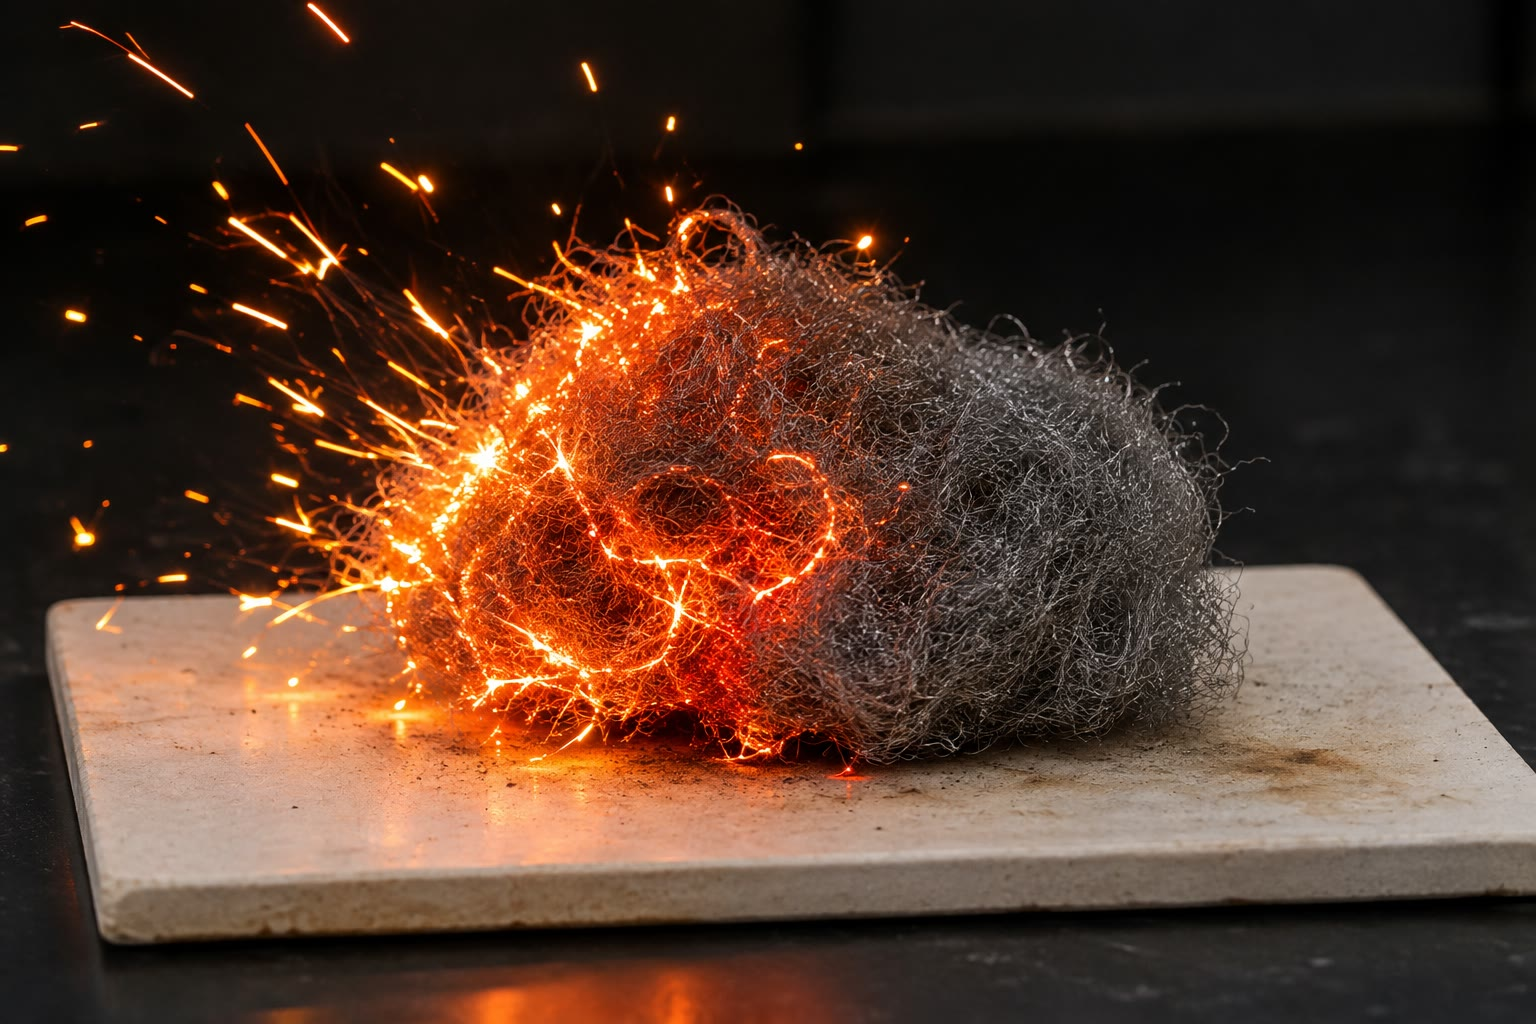
\includegraphics[width=0.5\linewidth]{images/book1/ai/g7-steel-wool-burning.jpg}

{\small 钢丝绒在实验室中燃烧：铁与氧气发生反应。}
\end{omfigure}

\section{文字表达式}

\begin{definition}[文字表达式]\label{def:g7:chemical-reactions:word-equation}
\emph{文字表达式}\index{文字表达式}用文字表示化学反应，
即在左边写出反应物的名称，并用 $+$ 连接，
再用箭头连接，右边写出生成物的名称。箭头读作
“反应生成”。
\end{definition}

\begin{example}[三个文字表达式]\label{ex:g7:chemical-reactions:three}
\begin{center}
\begin{tabular}{l}
碳 $+$ 氧气 $\longrightarrow$ 二氧化碳 \\[2pt]
甲烷 $+$ 氧气 $\longrightarrow$ 二氧化碳 $+$ 水 \\[2pt]
铁 $+$ 氧气 $\longrightarrow$ 氧化铁
\end{tabular}
\end{center}
\end{example}

\begin{method}[书写文字表达式]\label{met:g7:chemical-reactions:write}
\begin{enumerate}
  \item 找出反应物：即消失的物质。
  \item 找出生成物：即新生成的物质，通过检验加以确认。
  \item 反应物写在左边，生成物写在右边，
        中间用箭头连接，切勿使用等号。
\end{enumerate}
存在但不参与反应的物质——如火焰周围空气中的氮气——
不必写出。
\end{method}

\section{反应是原子的重新排列}

\begin{proposition}[原子被重新排列]\label{prop:g7:chemical-reactions:rearranged}
在化学反应中，反应物的分子被拆散，
原子以不同的方式重新结合，构成
生成物的分子。原子本身既不会产生，也不会消失：
同样的原子，数目相同，反应前后都存在。
\end{proposition}

\begin{example}[甲烷燃烧的分子变化]\label{ex:g7:chemical-reactions:methane}
燃气灶中的甲烷燃烧时，一个甲烷分子 \ce{CH4}
与两个氧分子 \ce{O2} 相遇，它们的原子重新排列，生成一个
二氧化碳分子 \ce{CO2} 和两个水分子 \ce{H2O}。
反应前：1 个碳原子、4 个氢原子和 4 个氧原子。反应后：1 个碳原子、4
个氢原子，以及 $2 + 2 = 4$ 个氧原子。没有原子损失，也没有
凭空出现。
\end{example}

\begin{omfigure}
\begin{tikzpicture}[font=\small]
  % methane
  \begin{scope}[xshift=0cm]
    \node[aC] (c) at (0,0) {};
    \node[aH] (h1) at (0,0.78) {}; \node[aH] (h2) at (-0.74,-0.3) {};
    \node[aH] (h3) at (0.74,-0.3) {}; \node[aH] (h4) at (0.2,-0.68) {};
    \begin{scope}[on background layer]
      \foreach \h in {h1,h2,h3,h4} \draw[bond] (c.center) -- (\h.center);
    \end{scope}
    \node at (0,-1.2) {1 甲烷};
  \end{scope}
  \node at (1.45,0) {$+$};
  % two oxygen molecules
  \foreach \y in {0.45,-0.45} {
    \node[aO] (a) at (2.4,\y) {}; \node[aO] (b) at (3.05,\y) {};
    \begin{scope}[on background layer]
      \draw[bond, line width=1.1pt] ([yshift=1.6pt]a.center) -- ([yshift=1.6pt]b.center);
      \draw[bond, line width=1.1pt] ([yshift=-1.6pt]a.center) -- ([yshift=-1.6pt]b.center);
    \end{scope}
  }
  \node at (2.72,-1.2) {2 氧气};
  \draw[->, thick, omProp] (3.8,0) -- (5.0,0);
  % carbon dioxide
  \begin{scope}[xshift=6.3cm]
    \node[aO] (a) at (-0.8,0) {}; \node[aC] (c) at (0,0) {}; \node[aO] (b) at (0.8,0) {};
    \begin{scope}[on background layer]
      \foreach \d in {-1.6,1.6} {
        \draw[bond, line width=1.1pt] ([yshift=\d pt]a.center) -- ([yshift=\d pt]c.center);
        \draw[bond, line width=1.1pt] ([yshift=\d pt]c.center) -- ([yshift=\d pt]b.center);}
    \end{scope}
    \node at (0,-1.2) {1 二氧化碳};
  \end{scope}
  \node at (7.8,0) {$+$};
  % two water molecules
  \foreach \x in {8.9,10.6} {
    \node[aO] (o) at (\x,0.2) {};
    \node[aH] (p) at (\x-0.58,-0.25) {}; \node[aH] (q) at (\x+0.58,-0.25) {};
    \begin{scope}[on background layer]
      \draw[bond] (o.center) -- (p.center); \draw[bond] (o.center) -- (q.center);
    \end{scope}
  }
  \node at (9.75,-1.2) {2 水};
  % atom counts
  \node[align=center, font=\footnotesize] at (1.5,-2.0) {反应前：1 C，4 H，4 O};
  \node[align=center, font=\footnotesize] at (8.5,-2.0) {反应后：1 C，4 H，4 O};
\end{tikzpicture}

{\small 甲烷燃烧，用分子模型表示：反应物中的原子
重新排列为生成物。
反应前后的原子均被计入。}
\end{omfigure}

\begin{remark}[分子的计数]\label{rem:g7:chemical-reactions:counting}
文字表达式没有说明有多少个分子参加反应。要表示这一点，
需在化学式前加上数字，写成化学方程式。
如何书写这类方程式、确定正确的数字，
将在后面的章节中学习。
\end{remark}

\section{练习}

\begin{exercise}[$\star$]\label{exo:g7:chemical-reactions:1}
判断下列变化是物理变化还是化学变化：
冰熔化、火柴燃烧、糖溶解、烤面包、铁钉生锈。
\end{exercise}

\begin{exercise}[$\star$]\label{exo:g7:chemical-reactions:2}
什么是化学反应的反应物和生成物？
\end{exercise}

\begin{exercise}[$\star$]\label{exo:g7:chemical-reactions:3}
写出碳在氧气中燃烧的文字表达式。
\end{exercise}

\begin{exercise}[$\star$]\label{exo:g7:chemical-reactions:4}
在文字表达式“铁 $+$ 氧气 $\longrightarrow$ 氧化铁”中，
指出反应物和生成物。
\end{exercise}

\begin{exercise}[$\star\star$]\label{exo:g7:chemical-reactions:5}
甲烷燃烧时，把冷玻璃片放在火焰上方，玻璃片上出现水雾；
收集到的气体使石灰水变浑浊。
这两项检验说明了哪些生成物？
\end{exercise}

\begin{exercise}[$\star\star$]\label{exo:g7:chemical-reactions:6}
锌与盐酸发生反应：锌逐渐消失，
放出氢气，氯化锌留在溶液中。写出
该反应的文字表达式。
\end{exercise}

\begin{exercise}[$\star\star$]\label{exo:g7:chemical-reactions:7}
观察甲烷燃烧的模型图。数一数反应前后
氢原子的数目。
\end{exercise}

\begin{exercise}[$\star\star$]\label{exo:g7:chemical-reactions:8}
虽然食盐溶于水后从视线中消失，
但为什么这不是化学反应？
\end{exercise}

\begin{exercise}[$\star\star$]\label{exo:g7:chemical-reactions:9}
一段木柴烧成了一小堆灰烬。请用“生成物”一词说明，
为什么灰烬比木柴轻得多。
\end{exercise}

\begin{exercise}[$\star\star$]\label{exo:g7:chemical-reactions:10}
氢气在氧气中燃烧，只生成水。写出文字表达式，
并说明用哪种检验可以确定生成物。
\end{exercise}

\begin{exercise}[$\star\star\star$]\label{exo:g7:chemical-reactions:11}
两个氢分子 \ce{H2} 与一个氧分子 \ce{O2} 反应，
生成两个水分子 \ce{H2O}。数一数反应前后
各种原子的数目，说明没有原子产生或消失。
\end{exercise}

\begin{exercise}[$\star\star\star$]\label{exo:g7:chemical-reactions:12}
一名学生把碳的燃烧画成：一个碳原子 $+$ 一个氧
分子 $\longrightarrow$ 一个二氧化碳分子和一个氧
原子剩余。这幅图画错了什么？
请用文字写出正确的画法。
\end{exercise}

\section{问题：燃气灶火焰中的变化}

\begin{problem}[{周末问题——燃气灶火焰中燃烧的是什么、生成了什么，
以及有多少个分子参加反应}]
\label{pb:g7:chemical-reactions:1}
厨房燃气灶用的燃气主要是甲烷 \ce{CH4}。在蓝色的
火焰中，甲烷与空气中的氧气反应。在实验室里，老师
老师把一个干燥的冷烧杯倒扣在这样的火焰上方，
持续几秒钟，然后将烧杯翻转，加入少量石灰水，
并振荡。

\medskip
\noindent\textbf{第一部分——反应物和生成物。}
\begin{enumerate}
  \item 写出该反应的两种反应物。
  \item 冷烧杯内壁出现液滴，取一滴液滴使无水硫酸铜
        变蓝。这说明生成了哪种产物？
  \item 石灰水变浑浊。这说明生成了另一种哪种产物？
  \item 空气中还含有氮气，它穿过火焰时
        不发生变化。氮气是反应物吗？它
        是否应写入文字表达式？
\end{enumerate}

\medskip
\noindent\textbf{第二部分——文字表达式。}
\begin{enumerate}[resume]
  \item 写出该反应的文字表达式。
  \item 甲烷的燃烧是物理变化还是
        化学变化？请给出两条理由。
  \item 写出该反应中四种物质的化学式。
\end{enumerate}

\medskip
\noindent\textbf{第三部分——数一数分子。}
每个燃烧的甲烷分子与两个氧分子反应，
生成一个二氧化碳分子和两个水分子。
\begin{enumerate}[resume]
  \item 数出一个甲烷
        分子和两个氧分子中的碳、氢、氧原子数（合计）。
  \item 数出一个二氧化碳分子和两个水分子中
        的原子数（合计）。你发现了什么？
  \item 火焰燃烧了 10 个甲烷分子，
        需用多少个氧分子？
  \item 生成多少个二氧化碳分子？
  \item 生成多少个水分子？
\end{enumerate}
\end{problem}
